\documentclass[11pt]{article}
\usepackage[margin=0.82in]{geometry}
\usepackage{amsmath,amssymb,amsthm,graphicx,microtype}
\usepackage[T1]{fontenc}
\usepackage{lmodern}
\usepackage[hidelinks]{hyperref}
\newtheorem{theorem}{Theorem}
\newtheorem{proposition}{Proposition}
\newcommand{\C}{\mathbb C}
\newcommand{\I}{\mathbf 1}
\title{A Scalar Counterexample to the Positive\\
Lower-Ratio Approximation Conjecture}
\author{Automatic math-discovery run \texttt{fa\_banach\_001}}
\date{August 11, 2026}

\begin{document}
\maketitle

\section*{Status}
Candidate full counterexample to the lower-ratio part of Remark~2 in
Chang's arXiv:2407.05062v1 \cite{Chang}.  The proof is exact and
one-dimensional.  Human review is recommended, chiefly to decide whether the
source intended an unstated strict-positivity hypothesis on the numerator.

\section*{Source problem}
Section~7.1 of the source permits an arbitrary real-valued continuous
function $f$ and a polynomial map $\Phi$ of the broad form in its Eq.~(10).
It asks for an invertible denominator $g$ and polynomial arguments satisfying
the single-operator upper and lower ratios (74)--(75), and the averaged
versions (81)--(82).  Remark~2 then says that the authors ``conjecture the
existence of function $g(\mathbf x)$ and polynomials in terms of $\Psi$ as
arguments'' for any prescribed $\alpha _1$ or $\alpha _2$ \cite[p.~29]{Chang}.
Both $\alpha _1$ and $\alpha _2$ are specified to be positive.

The relevant setup and four requirements are reproduced from PDF
pages~23--25, followed by Remark~2 on page~29.

\begin{center}
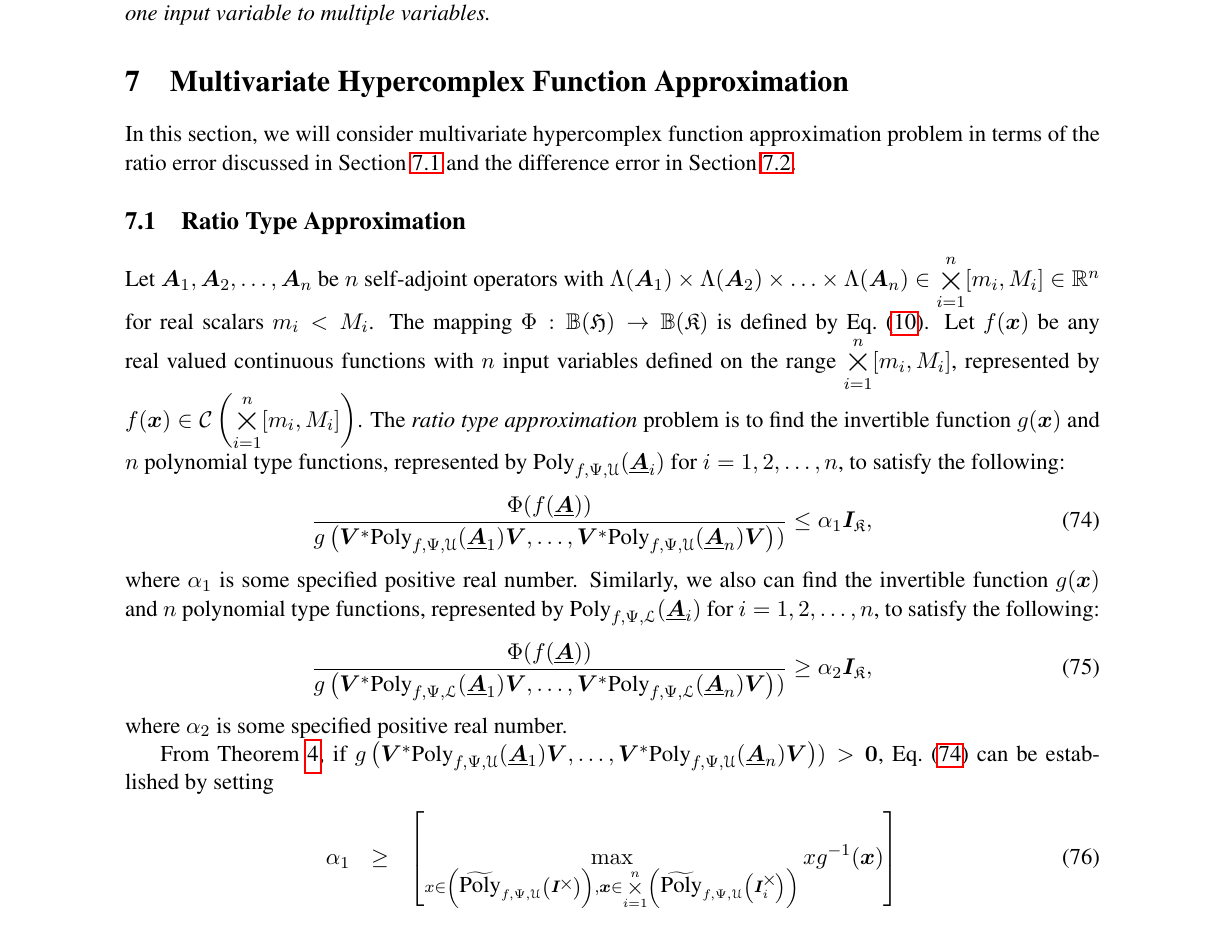
\includegraphics[width=0.96\textwidth]{figures/ratio_single_requirements.png}

\smallskip
{\small Source page 23: the single-operator requirements (74)--(75).}
\end{center}

\begin{center}
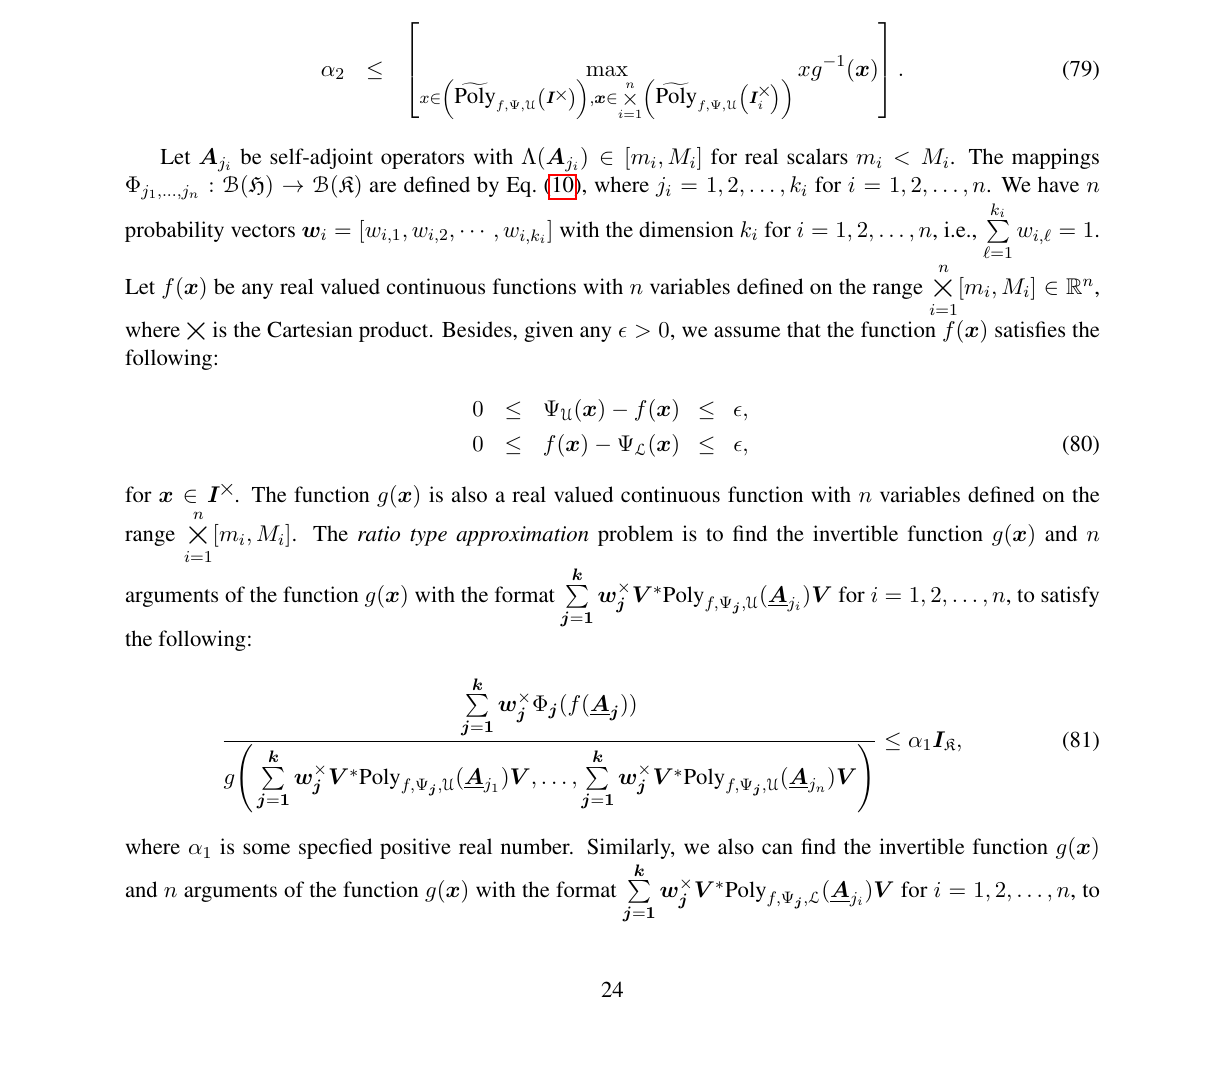
\includegraphics[width=0.96\textwidth]{figures/ratio_averaged_requirement_81.png}

\smallskip
{\small Source page 24: the averaged setup and requirement (81).}
\end{center}

\begin{center}
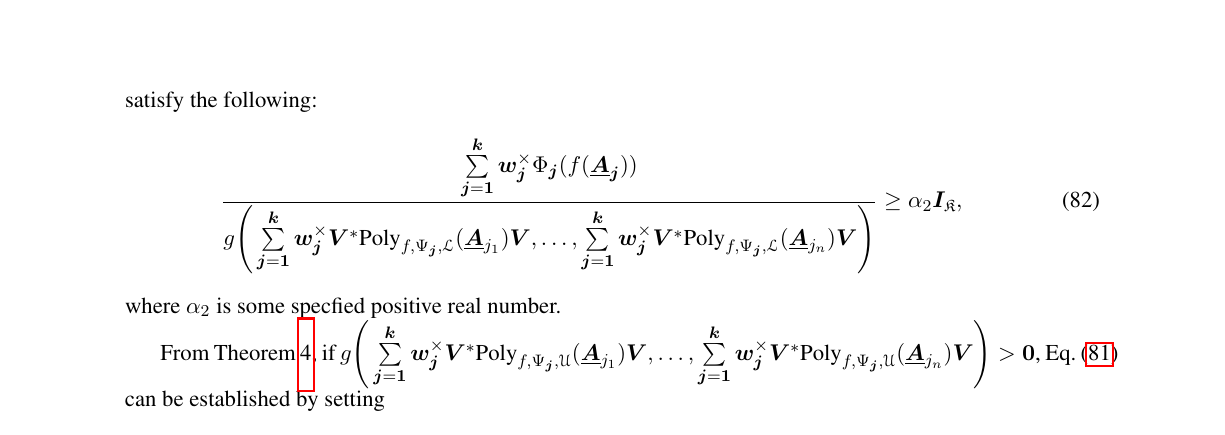
\includegraphics[width=0.96\textwidth]{figures/ratio_averaged_requirement_82.png}

\smallskip
{\small Source page 25: the averaged lower requirement (82).}
\end{center}

\begin{center}

\includegraphics[width=0.96\textwidth]{figures/open_problem_crop.png}

\smallskip
{\small Source page 29: Remark 2.}
\end{center}

\section*{Precise claim addressed}
The lower single-operator requirement is, in the scalar specialization,
\begin{equation}\label{eq:lower}
 \frac{\Phi(f(A))}{g(P_L(A))}\geq \alpha _2,
 \qquad \alpha _2>0,
\end{equation}
where $P_L(A)$ abbreviates the proposed lower polynomial argument and the
denominator is required to be invertible.  The averaged requirement replaces
the numerator and the argument by the weighted expressions in Eq.~(82).
Remark~2 asserts existence for arbitrary prescribed $\alpha _2$ in this
setup.  Refuting either lower requirement refutes that universal assertion.

\section*{Idea of the proof}
The polynomial maps admitted by the source can annihilate a strictly positive
input.  Choose $f\equiv1$ but take $\Phi(X)=X^2-X^3$, so that
$\Phi(f(A))=\Phi(1)=0$.  Changing $g$ or any of its polynomial arguments can
only change the denominator.  An invertible denominator cannot turn a zero
numerator into a strictly positive ratio.  Taking a one-term average makes
the averaged formula identical to the same scalar contradiction.

\section*{Counterexample}
\begin{theorem}\label{thm:counterexample}
For every $\alpha _2>0$, there are data satisfying the stated setup of
Section~7.1 for which no invertible $g$ and no choice of polynomial arguments
can satisfy Eq.~(75).  The same data, with a one-term average, also make
Eq.~(82) impossible.  Consequently the positive lower-ratio existence part
of Remark~2 is false as stated.
\end{theorem}

\begin{proof}
Take
\[
 n=1,\qquad \mathfrak H=\mathfrak K=\C,\qquad I=[0,1],
 \qquad A=\tfrac12,\qquad V=1,
\]
and let $f(x)=1$ on $I$.  Define the polynomial map
\begin{equation}\label{eq:phi}
 \Phi(X)=X^2-X^3.
\end{equation}
This is exactly of the source's Eq.~(10) form: take $a_2=1$, $a_3=-1$,
all other coefficients zero, and $V=1$.  The source expressly imposes no
linearity, positivity, or normalization constraint on this generalized
$\Phi$ \cite[p.~5]{Chang}.

For completeness, the sigmoid bracketing assumptions used in the surrounding
results are nonempty for these data.  Given $\varepsilon>0$, let
$\sigma(t)=(1+e^{-t})^{-1}$ and choose
$0<\delta<\min\{1,\varepsilon\}$.  Then
\[
 \Psi_U(x)=1+\delta\sigma(x),\qquad
 \Psi_L(x)=1-\delta\sigma(x)
\]
are linear combinations of sigmoids (use $1=2\sigma(0)$), remain strictly
positive on $I$, and satisfy
\[
 0\leq\Psi_U-f\leq\varepsilon,
 \qquad 0\leq f-\Psi_L\leq\varepsilon.
\]

Functional calculus gives $f(A)=1$.  Applying \eqref{eq:phi},
\begin{equation}\label{eq:zero}
 \Phi(f(A))=\Phi(1)=1^2-1^3=0.
\end{equation}
Now allow \emph{any} proposed lower polynomial argument $P_L(A)$ and
\emph{any} proposed $g$ for which the scalar denominator
$d=g(P_L(A))$ is invertible.  Thus $d\neq0$, but \eqref{eq:zero} yields
\[
 \frac{\Phi(f(A))}{g(P_L(A))}=\frac0d=0<\alpha _2.
\]
This contradicts \eqref{eq:lower} independently of how $g$ and $P_L$ are
chosen.

For Eq.~(82), take $k_1=1$, weight $w_{1,1}=1$, and the same $A$, $\Phi$,
$f$, and brackets.  Its weighted numerator is again $\Phi(f(A))=0$, so the
identical contradiction proves the averaged assertion.
\end{proof}

\section*{Structural obstruction}
The example is not an artifact of choosing an unfortunate scale for $g$.
It realizes the exact missing hypothesis.

\begin{proposition}\label{prop:obstruction}
Under the positive-denominator interpretation used in the source theorem,
if
\[
 G^{-1/2}YG^{-1/2}\geq\alpha I,
 \qquad G>0,\quad \alpha>0,
\]
then $Y\geq\alpha G>0$.  In particular, a singular numerator $Y$ can never
satisfy a positive lower-ratio bound.
\end{proposition}

\begin{proof}
Congruence by $G^{1/2}$ gives $Y\geq\alpha G$.  Since $G$ is positive and
invertible, its lower spectral bound is strictly positive, and hence so is
that of $Y$.
\end{proof}

The scalar construction in Theorem~\ref{thm:counterexample} avoids any
possible ambiguity about noncommutative quotient notation.  It shows that a
repair must at least restrict the allowed data so that $\Phi(f(A))$ has a
uniform positive lower bound.  That condition is absent from Remark~2.

\section*{Verification, scope, and novelty}
The accompanying script checks the scalar identity with exact rational
arithmetic for representative positive and negative nonzero denominators.
It is a sanity check only; the proof does not depend on computation.

This packet refutes the lower-ratio requirements (75) and (82), which is
enough to disprove Remark~2 as a universal existence claim for arbitrary
positive $\alpha _2$.  It does not claim that the upper-ratio requirement for
$\alpha _1$ is false.  It also does not resolve the separate difference-type
Remark~3; its displayed requirements contain a free scalar $x$ on the
right-hand side and need clarification before a precise universal statement
can be assessed.

A bounded novelty search on August 11, 2026 covered the run indexes, the exact
arXiv id and title, the phrases ``ratio type approximation'' and the
conjecture wording, and current web/arXiv results for the author and topic.
It found the source and mirrors but no later paper explicitly resolving
Remark~2.  Absence from that bounded search is not proof of novelty.

\section*{Human-review recommendation}
Send to human review.  The decisive checks are that Eq.~(10) really admits
\eqref{eq:phi}, and that the printed conjecture contains no strict-positivity
hypothesis on $\Phi(f(A))$.  If such a hypothesis was intended, it should be
stated as a repair; it is not part of the conjecture addressed here.

\begin{thebibliography}{1}
\bibitem{Chang}
S.-Y. Chang,
\emph{Generalized Multivariate Hypercomplex Function Inequalities and Their Applications},
arXiv:2407.05062v1 (2024),
\url{https://arxiv.org/abs/2407.05062}.
\end{thebibliography}

\end{document}
